%
% File acl2020.tex
%
%% Based on the style files for ACL 2020, which were
%% Based on the style files for ACL 2018, NAACL 2018/19, which were
%% Based on the style files for ACL-2015, with some improvements
%%  taken from the NAACL-2016 style
%% Based on the style files for ACL-2014, which were, in turn,
%% based on ACL-2013, ACL-2012, ACL-2011, ACL-2010, ACL-IJCNLP-2009,
%% EACL-2009, IJCNLP-2008...
%% Based on the style files for EACL 2006 by
%%e.agirre@ehu.es or Sergi.Balari@uab.es
%% and that of ACL 08 by Joakim Nivre and Noah Smith

\documentclass[11pt,a4paper]{article}
\usepackage[hyperref]{acl}

\usepackage{times}
\usepackage{amsmath}
\usepackage{url}
\usepackage{latexsym}
\usepackage{hyperref}
\usepackage[pdftex]{graphicx}
\usepackage{makecell}
\usepackage[utf8]{inputenc}
\usepackage[russian,english]{babel}
\usepackage{geometry}
\usepackage{pdflscape}
\usepackage{caption}
\usepackage{xcolor}
\usepackage{tabularx}

%\usepackage{showframe}
\renewcommand{\UrlFont}{\ttfamily\small}
\newcommand{\argmax}{\mathrm{argmax}}

% This is not strictly necessary, and may be commented out,
% but it will improve the layout of the manuscript,
% and will typically save some space.
\usepackage{microtype}

%\aclfinalcopy % Uncomment this line for the final submission
%\def\aclpaperid{***} %  Enter the acl Paper ID here

%\setlength\titlebox{5cm}
% You can expand the titlebox if you need extra space
% to show all the authors. Please do not make the titlebox
% smaller than 5cm (the original size); we will check this
% in the camera-ready version and ask you to change it back.

\newcommand\BibTeX{B\textsc{ib}\TeX}

\title{Quantifying Morphology in Latent Dirichlet Analysis Topic Models}

\author{Virginia Partridge \\
  University of Massachusetts Amherst\\
  \texttt{vcpartridge@umass.edu}
}
\date{}

\begin{document}
\maketitle
\begin{abstract}
    Latent Dirichlet Analysis (LDA) is a popular approach for topic modeling, frequently applied in many disciplines for exploring themes and trends in large document collections. Stemming or lemmatization are common pre-processing steps in preparing corpora for topic modeling, despite little evidence that these improve topic quality for English. Recent work has suggested post-processing topics so that they are more interpretable by end users may be a better approach.

    We present several metrics designed to quantify the morphological and lexical complexity of topics learned by LDA, with a focus on identifying topics that may benefit from post-processing. We then use these metrics to analyze LDA topic models trained with Gibbs sampling on Russian and German corpora, comparing the effects of different stemmers and lemmatizers.
    % TODO Summarize findings...
\end{abstract}

\section{Introduction}
Latent Dirichlet Analysis (LDA) is a widely adopted approach for unsupervised topic modeling and has been used across disciplines for exploring themes and trends in large document collections. LDA has been applied to explore the ever-growing variety of English and Russian text from online platforms and to analyze language changes in academic fields over time \cite{koltsova2013,mcfarland2013differentiating, vogel-jurafsky-2012-said, mitrofanova2015probabilistic}. Assuming a bag-of-words approach, LDA produces latent topics as multinomial distributions over words and each topic is viewed as being generated by a mixture of topics \cite{blei2003,steyvers2007probabilistic}.

However, what happens when words in this bag-of-words approach are themselves are complex? We turn to topic modeling on Russian, a flective language with rich paradigms for nouns, adjectives and verbs \cite{wade2020comprehensive}. Russian's inflectional morphology increases the sparsity of words' surface forms in the collection, but it's unclear to what extent this sparsity impacts the interpretability and usefulness of topics. Stemming and lemmatization treatments are typical text preprocessing steps for topic modeling, even for English, which has relatively little inflectional morphology, but there is a lack of empirical evidence that these treatments improve the models from the perspective of human interpretability or quantitative measures of topic quality \cite{schofield-mimno-2016-comparing}.

Furthermore, conflation of surface word forms may mask phenomena of interest to researchers. Topic modeling is a popular tool for exploring gender bias in corpora \cite{vogel-jurafsky-2012-said,devinney-etal-2020-semi}, and many languages, Russian included, have inflectional morphology that marks gender. By normalizing tokens to a single form, topics learned in LDA won't distinguish between Russian's feminine, masculine and neuter word forms, which may or may not be desirable depending on the domain and researchers' goals. The situation in Russian is even more nuanced than the oft cited English example ``apple'', the company, as opposed to ``apples'', the fruit \cite{schofield-mimno-2016-comparing}, as the different surface forms in Russian do share an underlying lexical word sense, but their variation results from requirements of the language's grammar.

In this work we explore baseline performance of LDA for topic modeling on a Russian literary corpus and report both quantitatively and qualitatively on the resulting topics. We first establish that topic modeling in Russian behaves similarly to English in terms of correlation with corpus metadata, regardless of the stemming or lemmatization approach. Without lexical conflation in Russian, we can imagine two possible extremes: either topic models learn lexeme-specific topics or they learn topics that demonstrate a particular grammatical feature in their morphology. By investigating topic models produced with no morphological preprocessing step, we see evidence for morphological features in topics and propose ways to quantify this relationship. These observations cast doubt on whether lemmatization is beneficial or if it obscures useful information. Finally, we address post-processing of topics' keywords as an alternative to aid with interpretability for end users.

\section{Related Work}
Probabilistic topic modeling has been applied on Russian text data from academic fields, social media, and Wikipedia articles \cite{mitrofanova2015probabilistic,koltsova2013,May2016AnAO}. Prior to the work on Wikipedia, little attention was given to the role of lemmatization on topic modeling in Russian, and corpora were lemmatized by default. In studying Russian Wikipedia, May et al. (2016) address the impact of lemmatization on topic interpretability via a word intrusion evaluation task, finding that lemmatization may be beneficial. However, they also suggest measuring the effects of lemmatization and do not rule out that lemmatizing in post-processing would also be effective.

The proposal for applying stemming in post-processing comes from work comparing the effects of various stemming approaches on English \cite{schofield-mimno-2016-comparing}. After comparing the relative strengths, qualitative and quantitative impacts of rule-based and context-based stemmers for English, it was concluded that stemmers do not emprically improve LDA topic models and may even hurt topic stability. Post-processing may still value from the perspective of topic interpretability, avoiding repeating surface forms of the same lexeme in topics' key word lists and presenting users with concise results.


\section{Background}

\subsection{Latent Dirichlet Analysis}
LDA uses the observed frequencies of vocabulary terms within documents to infer the \textit{latent}, or hidden, distributions of topics over words and topic assignments for each document. Once a number of topics $T$ is selected, the multinomial distributions $\phi_1,...\phi_T$ define the distribution of each topic $t$ over the vocabulary terms. Each $\phi_t$ is drawn from with a Dirichlet prior with concentration parameter $\beta$. Each document $d$ also has a multinomial distribution $\theta_d$ over the terms in the vocabulary, also drawn from a Dirichlet prior with concentration parameter $\alpha$. Viewing LDA as a generative process with a joint distribution of the observed and latent variables, find the $\phi_t$ and $\theta_d$ that maximize the likelihood of the corpus if you were to assign tokens to documents using the marginal distributions over topic assignments for the terms in each document. Gibbs Sampling allows estimation of the posterior for the joint topic distribution conditioned on the observed term frequencies by directly assigning topics to each token in the corpus, iteratively sampling topics and updating topic assignments
 \cite{steyvers2007probabilistic, blei2003,schofield-mimno-2016-comparing}.

Following Wallach et. al (2002), we will use a symmetric prior for $\beta$ and an asymmetric prior for $\alpha$ with the MALLET's Gibbs Sampling implementation to train topic models \cite{wallach2009rethinking,McCallumMALLET}. These parameters are optimized every 20 iterations after the first 50, the burn-in period. The Gibbs sampling implementation in MALLET allows us to directly inspect the topic assignments at the level of each token in a document.

\subsection{Framework for Morphological Complexity}
We will first clarify terms for discussing Russian's morphological paradigms, following frameworks for quantifying morphological complexity used in linguistics and computational linguistics \cite{baerman2015intro, cotterell-etal-2019-complexity}. We draw a distinction between \textit{derivational} morphology, the process by which new words are formed through changing meaning or part of speech, and \textit{inflectional} morphology, which can be simplistically understood as verb paradigms to capture subject-verb agreement or noun declensions for case and grammatical gender. For our purposes here, we are primarily interested in the equivalence classes formed by normalizing inflectional morphology, to use an English example, conflating ``respond" and ``responds", rather than ``respond" and ``responsiveness", although aggressive stemming methods will do both types of conflation.

In the word-based morphology framework, inflection is captured by triples consisting of the surface form (also called wordform) $w$, a lexeme  signifying the meaning and a slot $\sigma$, which can be understood as a set of ``atomic" units of morphological meaning, also called inflectional features \cite{aronoff1976word,sylak-glassman-etal-2015-language,cotterell-etal-2019-complexity}.
A lemma is the surface form used to look up the lexeme in a dictionary, such as the infinitive verb form. Measurements of the size of a lexeme's morphological paradigm capture \textit{enumerative complexity}, the number of distinct surface forms for a particular part-of-speech \cite{cotterell-etal-2019-complexity}. A lexeme's mapping between slots and the surface forms is not always straightforward outside the context of a sentence, as multiple slots may be realized with a single surface form (see the example of \foreignlanguage{russian}{большой} 'big' in table \ref{table:verbaspect}). This type of morphological complexity is called \textit{syncretism} and is common in Russian noun and adjective declensions \cite{baerman2015understanding,Milizia2015PatternsOS}.

There are two morphological tagsets commonly used for natural language processing of Russian. The first originates with Zalizniak's grammatical dictionary and is used in the Russian National Corpus. A detailed explanation of these tags can be found on the website of the Russian National Corpus\footnote{\url{https://ruscorpora.ru/new/en/corpora-morph.html}}. The second is the Universal Dependency tagset, which has been applied to the Russian dependency treebank SynTagRus \cite{Sharoff2011ThePP,lipenkova-soucek-2014-converting,mcdonald-etal-2013-universal}. Both of these tagsets express slots as a list of grammatical features and the two tagsets can be mapped to each other, although, as we shall see, their conflation classes (assigned lemmas) for Russian verbs differ significantly.

\section{Methods}
\subsection{Stemmers and Lemmatization Treatments}
\label{sec:stemmers}
Following Schofield and Mimno (2016), we distinguish between rule-based stemmers, which are deterministic, but only remove endings and do not map to lemmas, and context-based lemmatizers, which rely on a dictionary of word forms paired with outputs from a part-of-speech tagger to produce lemmas \cite{schofield-mimno-2016-comparing,Sharoff2011ThePP}. Rule-based methods make no distinction between inflectional and derivational morphological processes, leading to word types, conflation classes of terms, whose original surface forms may cover several lemmas.

\textbf{Truncation:} This simple baseline method trims surface forms to the first $n$ characters \cite{schofield-mimno-2016-comparing}. We truncate with $n=5$.

\textbf{Snowball Stemmer:} This stemmer was introduced as a rigorous framework for implementing stemming algorithms for a variety of languages. We utilize the NLTK implementation\footnote{\url{https://www.nltk.org/api/nltk.stem.html}} with the original rules for Russian\footnote{\url{http://snowball.tartarus.org/algorithms/russian/stemmer.html}} \cite{snowball}.


\textbf{Mystem:} This Yandex-owned tool is the most popular Russian lemmatizer and can be used without part-of-speech tags. Pairing a finite state machine algorithm for stemming with the Zalizniak grammatical dictionary for morphological tags, this system outputs a list of possible lemmas and slots for a given token input. The system also produces probabilities for each lemma and slot based on word frequency statistics, although the source corpus for these probabilities is not clear \cite{Segalovich2003AFM}. This is not truly a context-based lemmatizer, as it does not use part-of-speech tags to disambiguate between lemmas or to assign a single slot to a syncretic surface form, but the word frequencies do represent some kind of contextual prior. We use the python wrapper for Mystem, pymystem3\footnote{\url{pythonhosted.org/pymystem3/pymystem3.html}}. Notably, Mystem is as fast as the Snowball stemmer, while producing a normalized lemma form that is more interpretable for users. All slot and lemma entropy measurments produced in this paper are based on Mystem's morphological analysis for the most likely lexeme of the surface form.


\textbf{Stanza:} This toolkit implements full neural pipelines for processing raw text, including tagging morphological features using bidirectional long short-term memory networks and lemmatizing an ensemble of dictionary based and seq2seq methods \cite{qi2020stanza}. Because each step of the pipeline depends on the output of the previous step, in order to use Stanza for morphological tagging and lemmatization, we also use its tokenization and sentence-splitting. We use the Stanza model trained on the SynTagRus treebank\footnote{\url{https://universaldependencies.org/treebanks/ru_syntagrus/index.html}}. Unlike Mystem, Stanza always produces a single lemma and morphological slot, the disambiguation step is included within the model.

Other well-known lemmatizers for Russian include TreeTagger, CSTLemmatiser, pymorphy2 \cite{May2016AnAO,Sharoff2011ThePP,pymorphy2}. We opted not to use these here due to time constraints, as they are either difficult to install (TreeTagger, CSTLemmatiser) or very slow (pymorphy2).
\subsection{Evaluation metrics}
When it comes to topic modeling on Russian, we would like to quantify the trade-offs between topic interpretability and loss of information that is linked to a surface form's morphology. We can apply Mystem or Stanza to retrieve the most likely morphological analysis for a surface form $w$ in the vocabulary $V$ to find a lemma $\ell_w$ and slot $\sigma_w$. Using the token-level topic assignments from Gibbs Sampling as our surface form $w$, we follow Thompson and Mimno (2018) in viewing single topic assignments for each surface form as a data table with columns: surface form $w$, topic assignment $z$, slot $\sigma$, lemma $\ell$. For a given topic $k$, we obtain the joint count of the slots for the topic $N(\sigma, k)$, the counts of the lemmas for a topic $N(\ell, k)$ and the marginal count variable for a topic $N(k)$. Also note that $\argmax_{w \in V} N(w, k)$ denotes the top key words or surface forms for the topic.

\textbf{Morphological slot entropy:} The goal of this metric is to measure the concentration of slots within a given topic, a proxy for the enumerative complexity of the topic. Does a topic have a concentration of only a few morphological features or does it have a wide spread of the language's inventory of features? This metric is similar to Author Entropy discussed in Thompson and Mimno (2018), where the morphology of the language is the metadata we are attempting to capture, rather than the author of a document \cite{Thompson2018AuthorlessTM}. Topics that have low slot entropy would contain wordforms with the same grammatical features, for example different verbs conjugated in the first-person singular form or nominative case masculine nouns.
\begin{flalign}
    H(\sigma|k) &= \sum_\sigma P(\sigma|k) \log_2 P(\sigma|k) \\ \nonumber&= \sum_\sigma \frac{(N(\sigma, k))}{N(k)} \log_2 \frac{(N(\sigma, k))}{N(k)}
\end{flalign}

\textbf{Lemma entropy:} Similarly, we may want to know when a topic is dominated by a single lexeme, containing many grammatical forms of a single lexeme, but few other lexemes. For example, a topic may have many counts of different surface forms for each declension of a particular noun, its nominative, accustive, dative, etc... forms or even high counts for a single surface form, but relatively low counts of surface forms for any other lemma. Topics with very low lemma entropy may not be particularly useful to end users, as they reflect lexical and grammatical information known to every speaker of the language, but may not provide specific information about the corpus, other than the presence of a particular lexeme.
\begin{flalign}
    H(\ell|k) &= \sum_\ell P(\ell|k) \log_2 P(\ell|k) \\ \nonumber&= \sum_\ell \frac{(N(\ell, k))}{N(k)} \log_2 \frac{(N(\ell, k))}{N(k)}
\end{flalign}

\textbf{Ratio of slots to top $n$ key terms:} Here we are capturing whether a topic makes a particular grammatical feature obvious when results are displayed to the user. Although this doesn't account for the case when paradigms are syncretic on different dimensions, for example comparing first declension to third declension nouns \cite{wade2020comprehensive}, when this value is low, it suggests that the user will notice some sort of grammatical pattern within the topics.
\begin{flalign}
    R_\sigma(k) &= \frac{|\{\sigma_w | w \in  \{n \, \mathrm{largest} N(w, k)\} \}|}{n}
\end{flalign}


\textbf{Ratio of lemmas to top $n$ key terms:} This metric is targeted at understanding how concise the presentation of a topic's key terms is to a user. When the value is close to 1, each surface form presented to the user represents a unique lexeme. When this value is low, different forms of the same lexeme are repeated, the situation that has motivated the use for lemmatization or stemming to begin with.
\begin{flalign}
    R_\ell(k) &= \frac{|\{\ell_w | w \in \{n \, \mathrm{largest} N(w, k)\}\}|}{n}
\end{flalign}

\textbf{Type-token ratio:} Following Schofield and Mimno (2016), this corpus-level metric measures a stemmer or lemmatizer's conflation strength. It is found by taking the ratio of the number of word-type equivalence classes produced by the treatment (the post-treatment vocabulary size $|V|$) to the token counts for the corpus \cite{schofield-mimno-2016-comparing}.

\textbf{Character-token ratio:} This metric, also from Schofield and Mimno (2016), measures the aggressiveness of stemmers in trimming surface forms to a root form. It measures the average length of the tokens in the corpus after the stemming treatment. Because lemmatizers map surface forms to a normalized lemma instead, this metric isn't as meaningful for lemmatization.

\textbf{Author entropy:} Determining whether the topics correlate with known metadata provides a sanity check on the models. This metric, introduced by Thompson and Mimno (2018) measures how evenly a topic's tokens are spread across authors. We should expect to see both author-specific topic and general topics that are common to many authors \cite{Thompson2018AuthorlessTM}.

\textbf{Exclusivity:} Exclusivity quantifies the relative uniqueness of the top keywords in a topic. It is high when the terms most frequently generated by a topic are rarely generated by other topics in the model \cite{bischof2012exclusivity}.


\begin{table*}[th!]
    \centering
    \resizebox{\textwidth}{!}{\begin{tabular}{|l|r|r|r|r|r|}
    \hline
    \thead{\textbf{Stemming/Lemmatization}\\\textbf{Treatment}} & \thead{\textbf{Unpruned number}\\\textbf{of tokens}} & \thead{\textbf{Unpruned} \\\textbf{vocabulary size}} & \thead{\textbf{Number of tokens}\\\textbf{after pruning}} & \thead{\textbf{Vocabulry size}\\\textbf{after pruning}} & \thead{\textbf{Processing time for}\\\textbf{treatment (minutes)}}\\\hline
    No treatment & 6081210 & 319459 & 3321349 & 80540 &-\\\hline
Pymystem3 & 6084073 & 80163 & 2976804 & 32648 & 4.7 \\\hline
Snowball & 6081203 & 108533 & 3070870 & 35938 & 5 \\\hline
Stanza & 6097070 & 119602 & 2980649 & 38435 & 211.2 \\\hline
Truncate to 5 & 6081210 & 59469& 3357584 & 27994 & 0.25 \\\hline
    \end{tabular}}
    \caption{Token level corpus statistics for each lemmatization and stemming treatment. Differences in unpruned token counts are due to Pymystem3 and Stanza using their own tokenization and Snowball normalizing some single characters to empty strings.}
    \label{table:corpus}
\end{table*}

\begin{figure*}[th!]
    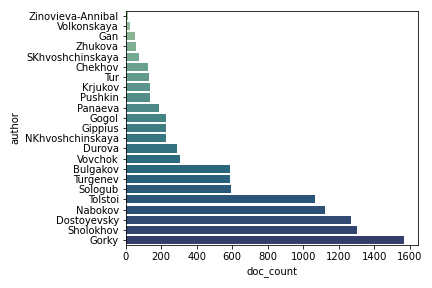
\includegraphics[width=0.5\textwidth]{document_count_by_author.png}
    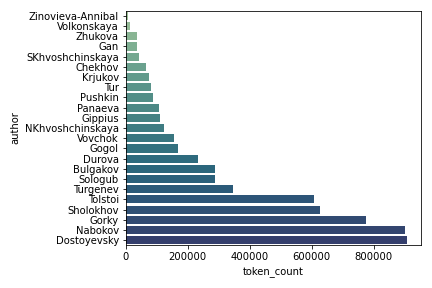
\includegraphics[width=0.5\textwidth]{token_count_by_author.png}
    \caption{The number of documents per author used to train topic models (left) and the token counts by author before pruning (right).}
    \label{fig:docsByAuthor}
\end{figure*}

\textbf{Coherence:} We additionally report coherence in figure \ref{fig:mallet_metrics_figs}. A measure of topic quality that relies on document co-occurence frequencies of word types, coherence has been reported to agree with human evaluations of topic quality \cite{mimno2011optimizing}. However, further work is required to adjust this measurement for the smaller vocabulary sizes resulting from conflation treatments \cite{schofield-mimno-2016-comparing}. The coherence results reported here cannot be interpreted as evidence for lemmatization helping or hurting the models' quality.

\section{Corpus}
The selected RussianNovels\footnote{\url{https://github.com/JoannaBy/RussianNovels}} corpus is a collection of 101 Russian literary works from the 19th and 20th centuries by 23 authors. The collection primarily consists of novels and novellas, but there are some plays (Chekhov and Sologub) and short stories (Gogol) as well. Duplicated works and multiple versions of the same work by different translators were removed. The deduplicated version of the corpus is available on Github \footnote{\url{https://github.com/ginic/RussianNovels/tree/cleanups}} with a change log.

Each work was subdivided into passages at least 500 tokens long, where tokens are determined by a simple non-whitespace pattern. This resulted in a corpus of 10,305 documents, broken down by author in figure \ref{fig:docsByAuthor}. Next, the corpus was re-tokenized using a regular expression capturing strings of alphabet characters of any length, with punctuation allowed between alphabet characters. Token-level statistics are given in table \ref{table:corpus}. We produced separate versions of the corpus for each treatment described in section \ref{sec:stemmers}. After conflation treatments, the resulting terms were pruned to a maximum document frequency of 25\% of the corpus and minimum term frequency of 5 occurences in the entire corpus. We chose these pruning settings as a reasonable alternative to manually determining a stopword list, as that process can be challenging and subjective \cite{schofield-etal-2017-pulling}.


\begin{figure*}[th]
    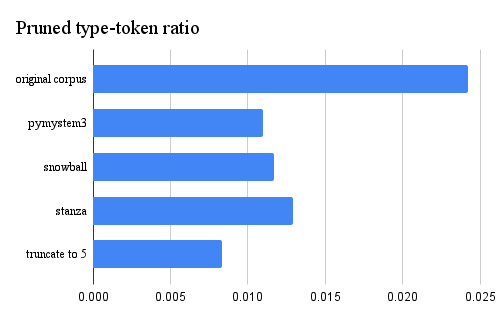
\includegraphics[width=0.5\textwidth]{pruned_type_token_ratio.png}
    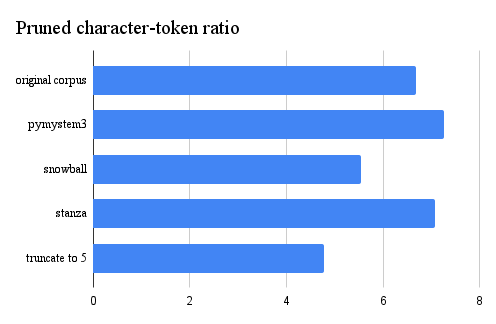
\includegraphics[width=0.5\textwidth]{pruned_character_token_ratio.png}
    \caption{The ratio of word types to tokens for each conflation treatment after the vocabulary is pruned is shown left and demonstrates the strength of conflation method in reducing the vocabulary. Character to token ratio shows lemmatization returns longer normalized strings, while stemming shortens them.}
    \label{fig:conflation_merics}
\end{figure*}


\section{Results}
After preprocessing the corpus using each stemmer or lemmatizer, we trained 5 models for each number of topics $T\in \{50, 100, 250, 500\}$. We also trained models on the corpus with no preprocessing treatment at all other than pruning and performed post-lemmatization on these models, using Mystem to produce topics with lemmas as the associated terms rather than surface-forms.


\begin{figure*}[t]
    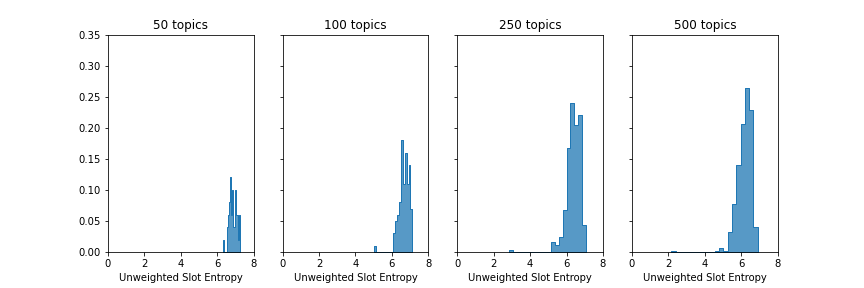
\includegraphics[width=0.5\textwidth]{unweighted_slot_entropy.png}
    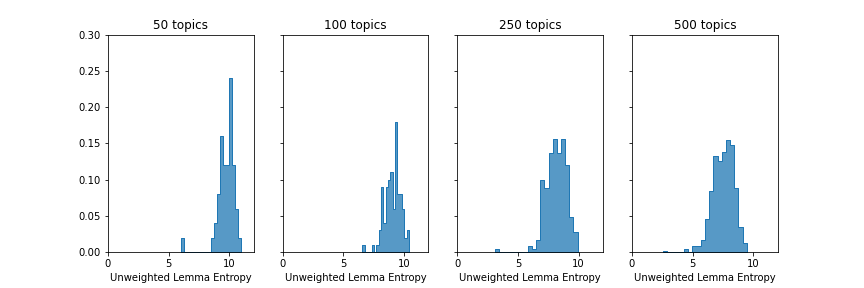
\includegraphics[width=0.5\textwidth]{unweighted_lemma_entropy.png}
    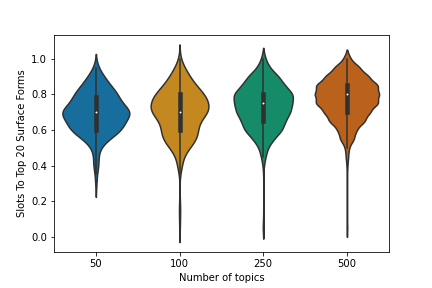
\includegraphics[width=0.5\textwidth]{slots_to_top_20_surface_forms.png}
    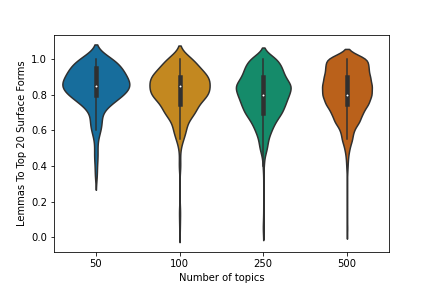
\includegraphics[width=0.5\textwidth]{lemmas_to_top_20_surface_forms.png}
    \caption{Values of metrics that capture morphological information in topics. These results are for topic models trained on the untreated corpus.}
    \label{fig:slot_lemma_figs}
\end{figure*}


\subsection{Qualitative Observations}
At the most basic level, we want to check to what extent topic modeling on this Russian literary corpus produces sensible results, showing some topics that correlate with metadata and others that capture general themes not specific to a particular author or time period. Author entropy does not directly measure model quality, in fact users often want topic models not correlated with known metadata \cite{Thompson2018AuthorlessTM}. However, it can at least reassure us that LDA performs on Russian in a way that is expectedly similar to English. Both the author correlation measures plotted in Appendix \ref{sec:author} show that stemming and lemmatization do not significantly affect whether author-specific topics or cross-cutting topics are learned, regardless of the number of topics.

Anecdotal analysis of topics' keywords also confirms topics obviously associated with specific authors and coherent general topics with a unified theme like `school', `travel', or `nature'. Some examples are described in detail in appendices \ref{sec:sample_original_topics} and \ref{sec:preprocessed_topics}. The models trained on untreated data also learn topics that are specific to particular morphological features, which we will revisit in detail in \ref{sec:slot_meaning}.

\subsection{Lemmatizer Choice Matters}
When examining the relative strengths of the stemmers and lemmatizers, laid out in figure \ref{fig:conflation_merics}, functional differences between the two lemmatizers are revealed. As expected, truncation, having the least type-token ratio, is the most aggressive treatment in terms of producing the largest word-type equivalence classes. The surprise is that Mystem is the next most aggressive, followed by Snowball, then Stanza. Since both Mystem and Stanza map surface forms to a normalized dictionary lemma, we expect them to be roughly equivalent in conflation strength.


This seemingly counter-intuitive result exposes a difference in the way that Mystem and Stanza handle verbal aspect. Nearly all Russian verbs have two infinitive forms, one for the imperfective aspect and one for the perfective aspect \cite{wade2020comprehensive}. Mystem treats all conjugations of the both imperfective and perfective aspects as surface forms of the same lexeme, mapping to the imperfective inifitive as the lemma. In contrast, Stanza maps to separate lemmas, imperfective forms to the imperfective infintive and perfective forms to the perfective infinitive. A clarifying example is given in table \ref{table:verbaspect}. As a non-native speaker, it's difficult predict what impact this distinction would have on topic interpretability, but the takeaway is that not all lemmatizers are equal. The choice of lemmatizer is not obvious and requires consideration of how the implementation groups the language's grammatical features and which grammatical features matter in the corpus domain.



\begin{center}
    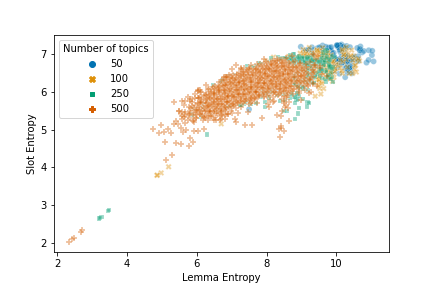
\includegraphics[width=0.5\textwidth]{lemma_slot_entropy_scatter.png}
    \captionof{figure}{Lemma entropy vs slot entropy for models trained without lemmatization. The seemingly direct relationship between them is due to Mystem expressing syncretism.}
    \label{fig:lemma_vs_slot_entropy}
\end{center}


\subsection{Meaning and Utility of Slot Measures}
\label{sec:slot_meaning}
Another result appearing contradictory at first glance is that slot entropy grows with lemma entropy for a topic. Given the initial assumption that lemmatization is done to remove redundant surface forms within a topic, we might expect that topics with low lemma entropy would have high slot entropy, a situation where topics are represented by many surface forms of a few lexemes. Conversely, when there are many lexemes, high lemma entropy, we might expect some repeated morphological forms, low slot entropy. Contrary to our expectation of an inverse relationship between lemma entropy and slot entropy, figure \ref{fig:lemma_vs_slot_entropy} shows a more direct relationship. This may be partially explained by Mystem's behaviour with respect to syncretism. Recall that Mystem's morphological analysis does not disambiguate in cases where the surface form is syncretic, it simply provides all possible analyses. When a topic covers more lexemes, there are also more opportunities for those lexemes to follow different morphological paradigms and patterns of syncretism. When Mystem is used to analyze topics, the number of slots for a topic will increase as the variety of declension and conjugation types in the topic increases. Because we are not disambiguating the morphological tags based on context, the slot entropy measurement reflects Russian's syncretism in addition to the grammatical features captured for the topic.

Despite the ambiguity around the true morphological features of each tag, the slot entropy and ratio measures produced from the Mystem representation is useful when it is low. Take the examples from a 100 topic model in appendix \ref{sec:sample_original_topics}, table \ref{table:sample_original_topics}. Topics that consist mostly of non-Russian terms, such as the `French' topic E, will have extremely low slot entropy and lemma entropy, since every term is assigned as the same \textit{UNKNOWN} slot and \textit{UNKNOWN} lemma, making it easy to identify these kinds of topics which aren't usually interesting to users.

The more interesting case is when slot entropy is low, but not a total outlier. For 100 topic models, the median value for slot entropy is about 6.5, as shown in figure \ref{fig:slot_lemma_figs}. The example topics D and F have some of the lowest slot entropy measures for the model from which they were selected, but have high lemma to keyword ratios, so there are almost no repeated lemmas within each topic. Topic D consists almost entirely of verbs in the past tense feminine form and F of verbs in the second-person singular, including some overlapping lexemes, `to talk',`to ask', `to sit', `to look' and `to begin'. Topic H also has some overlap with these lemmas, but in the past tense masculine form. If these topics were post-stemmed to a normalized form without considering the stem entropy, they would become nearly indistinguishable, a confusing situation to present to users. When stemming is done in preprocessing, it becomes impossible to learn these kinds of morphologically differentiated topics.

Whether users desire topics that reflect grammatical information, as opposed to topics split strictly on word sense relatedness, depends on the use case and domain, but slot entropy, even with ambiguous tags, can help to uncover such topics when there is no preprocessing. Since resources may not be available for a full morphological analysis of a large corpus, or you may only have topic keywords out of context, it's reassuring that slot entropy has meaning despite ambiguity.

\begin{center}
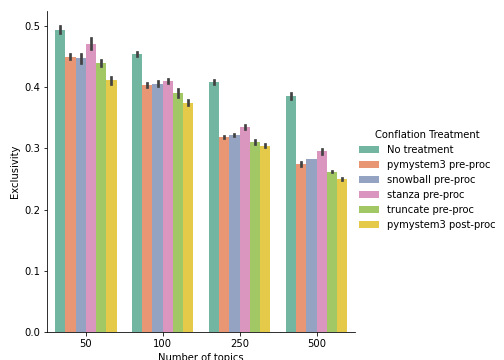
\includegraphics[width=0.5\textwidth]{exclusivity.png}
\captionof{figure}{Average exclusivity of topics with over all experiments for each conflation treatment.}
\label{fig:exclusivity}
\end{center}

\subsection{Models Don't Learn Lexeme-Specific Topics}
The motivation behind post-stemming is to prevent showing users topics that consist of multiple forms of the same lemma. We are able to identify topics that would benefit from post-stemming by using the topics using the ratio of lemmas to keywords. Take topics I and J in appendix \ref{sec:appendix_morph} figure \ref{table:sample_original_topics}, which have the second and third lowest lemma to keyword ratios of the 100 topic model investigated. Topic I has forms of the possessive pronoun \foreignlanguage{russian}{мой} repeated 12 times, making it difficult to interpret in any way. After post-stemming, it becomes obvious that this topic contains common words and isn't coherent. Topic J is clearly about school and school children, but there are redundant forms of `boy' and `school'. By post-lemmatizing, more related words, like `principal' and `student', are revealed.

These are clear cases where post-lemmatizing is useful, but the problem doesn't seem to be common. The average lemma to keyword ratio across all numbers of topics is around 0.8, meaning 16 of the 20 keywords are unique. Having such a low proportion of repeated keywords seems tolerable. Additionally, figure \ref{fig:exclusivity} demonstrates post-lemmatizing reduces exclusivity significantly. If lexemes were concentrated within the keywords of a single topic, then there shouldn't be such a large reduction in exclusivity. Coupled with the earlier observation that models do learn topics that express morphological features, a blanket application of post-lemmatization seems unwise, although applying it selectively based on some lemma to keyword threshold may be appropriate.

\section{Conclusions}
Anecdotally, LDA produces topic models that largely appear coherent and reasonable for this Russian literary corpus. Regardless of which conflation treatment is used, and even if none is used, both author-specific topics and thematic topics are found. Through morphological analysis of the terms for each topic and using a measure of morphological slot entropy, we established that models trained on corpus without preprocessing can also capture specific grammatical features. Topics with repeated surface forms of the same lemma are also present, but may not pose as large a challenge to usability as previously believed. Although post-lemmatizing provides clean, concise topic keywords, it obscures any grammatical information encoded in topics, which may lead to more confusion for users. We suggest that post-lemmatizing may be applied selectively to topics with a low ratio of lemmas to top keywords.

\section{Future Work}
More rigorous empirical comparisons are needed to discern the statistical differences between topic models under different stemming and lemmatization approaches. First, this requires revisiting the vocabulary pruning approach. Although using term and document frequency thresholds avoided the subjectivity of building a stopword list, not having a fixed vocabulary shared between the models over the various conflation methods made it difficult to compare models produced from post-processing, preprocessing, and the original untreated corpus. Fixing the vocabulary will allow us to compare topics empirically using measures of coherence, stability and variation of information.

Having uncovered Mystem's ambiguity with respect to syncretism, we would like to use a context-aware tagger, such as Stanza or TreeTagger, to gain more insight into what grammatical features topics may be capturing. This could also be explored using a corpus with manually annotated morphological tags. OpenCorpora\footnote{\url{opencorpora.org}} and the Russian National Corpus are good candidates for further exploration. These corpora also contain news and legal subsections, allowing us to ascertain whether our findings hold outside of the literary domain.

\bibliographystyle{acl_natbib}
\bibliography{references}

\appendix
\onecolumn
\section{Author Correlation Metrics with Conflation Treatments}
\label{sec:author}
\begin{center}
    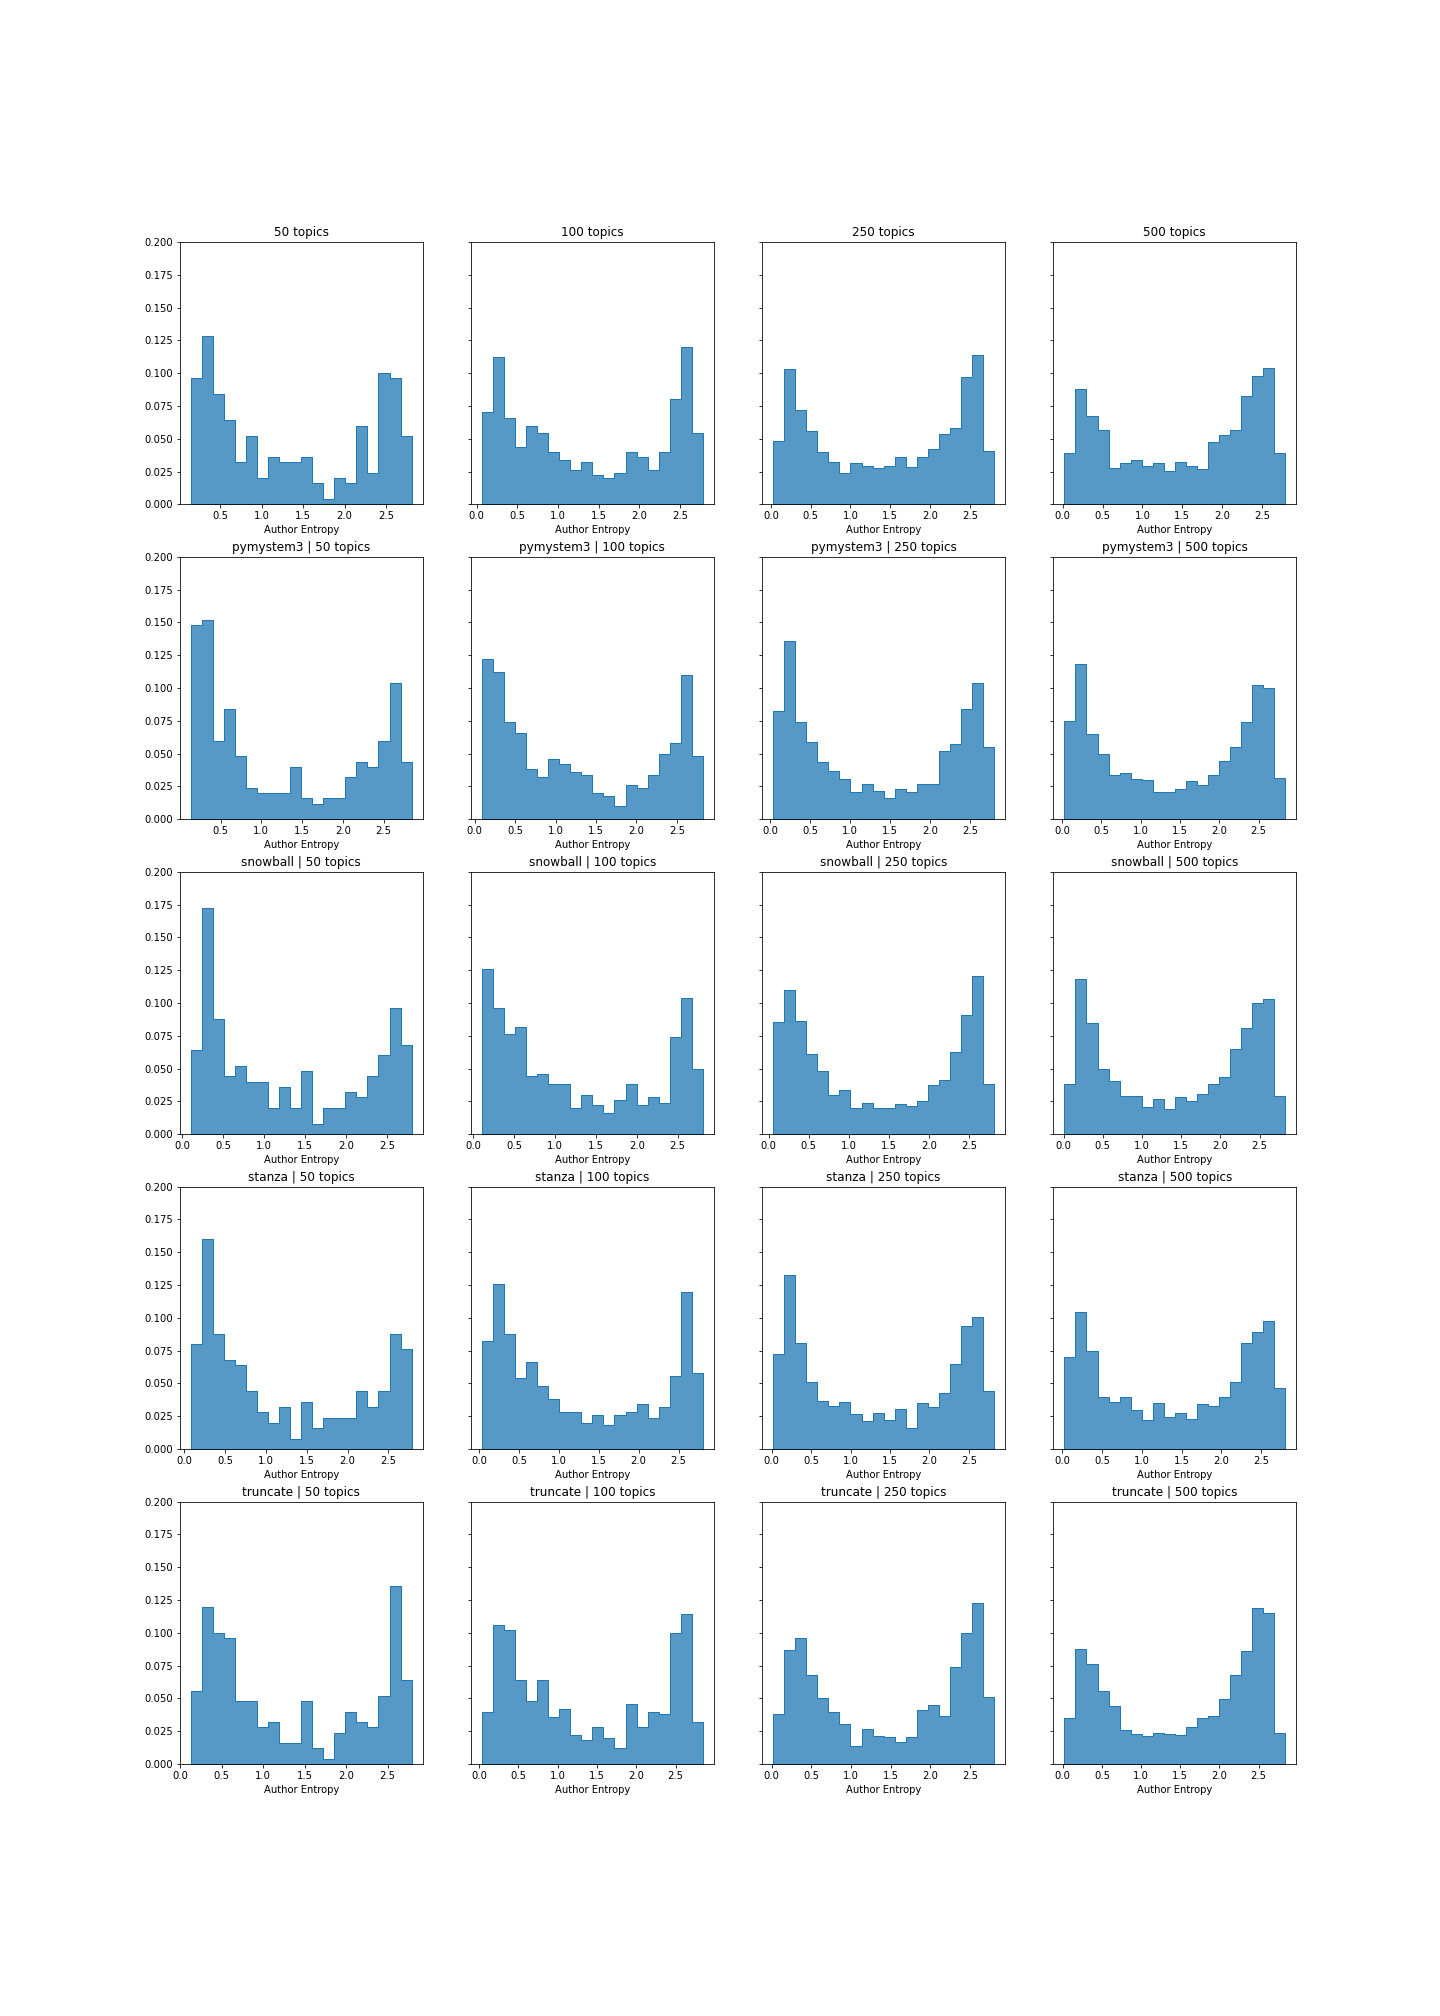
\includegraphics[width=\textwidth]{AuthorEntropy.png}
    %\includegraphics[width=\textwidth]{BalancedAnthors.png}
    %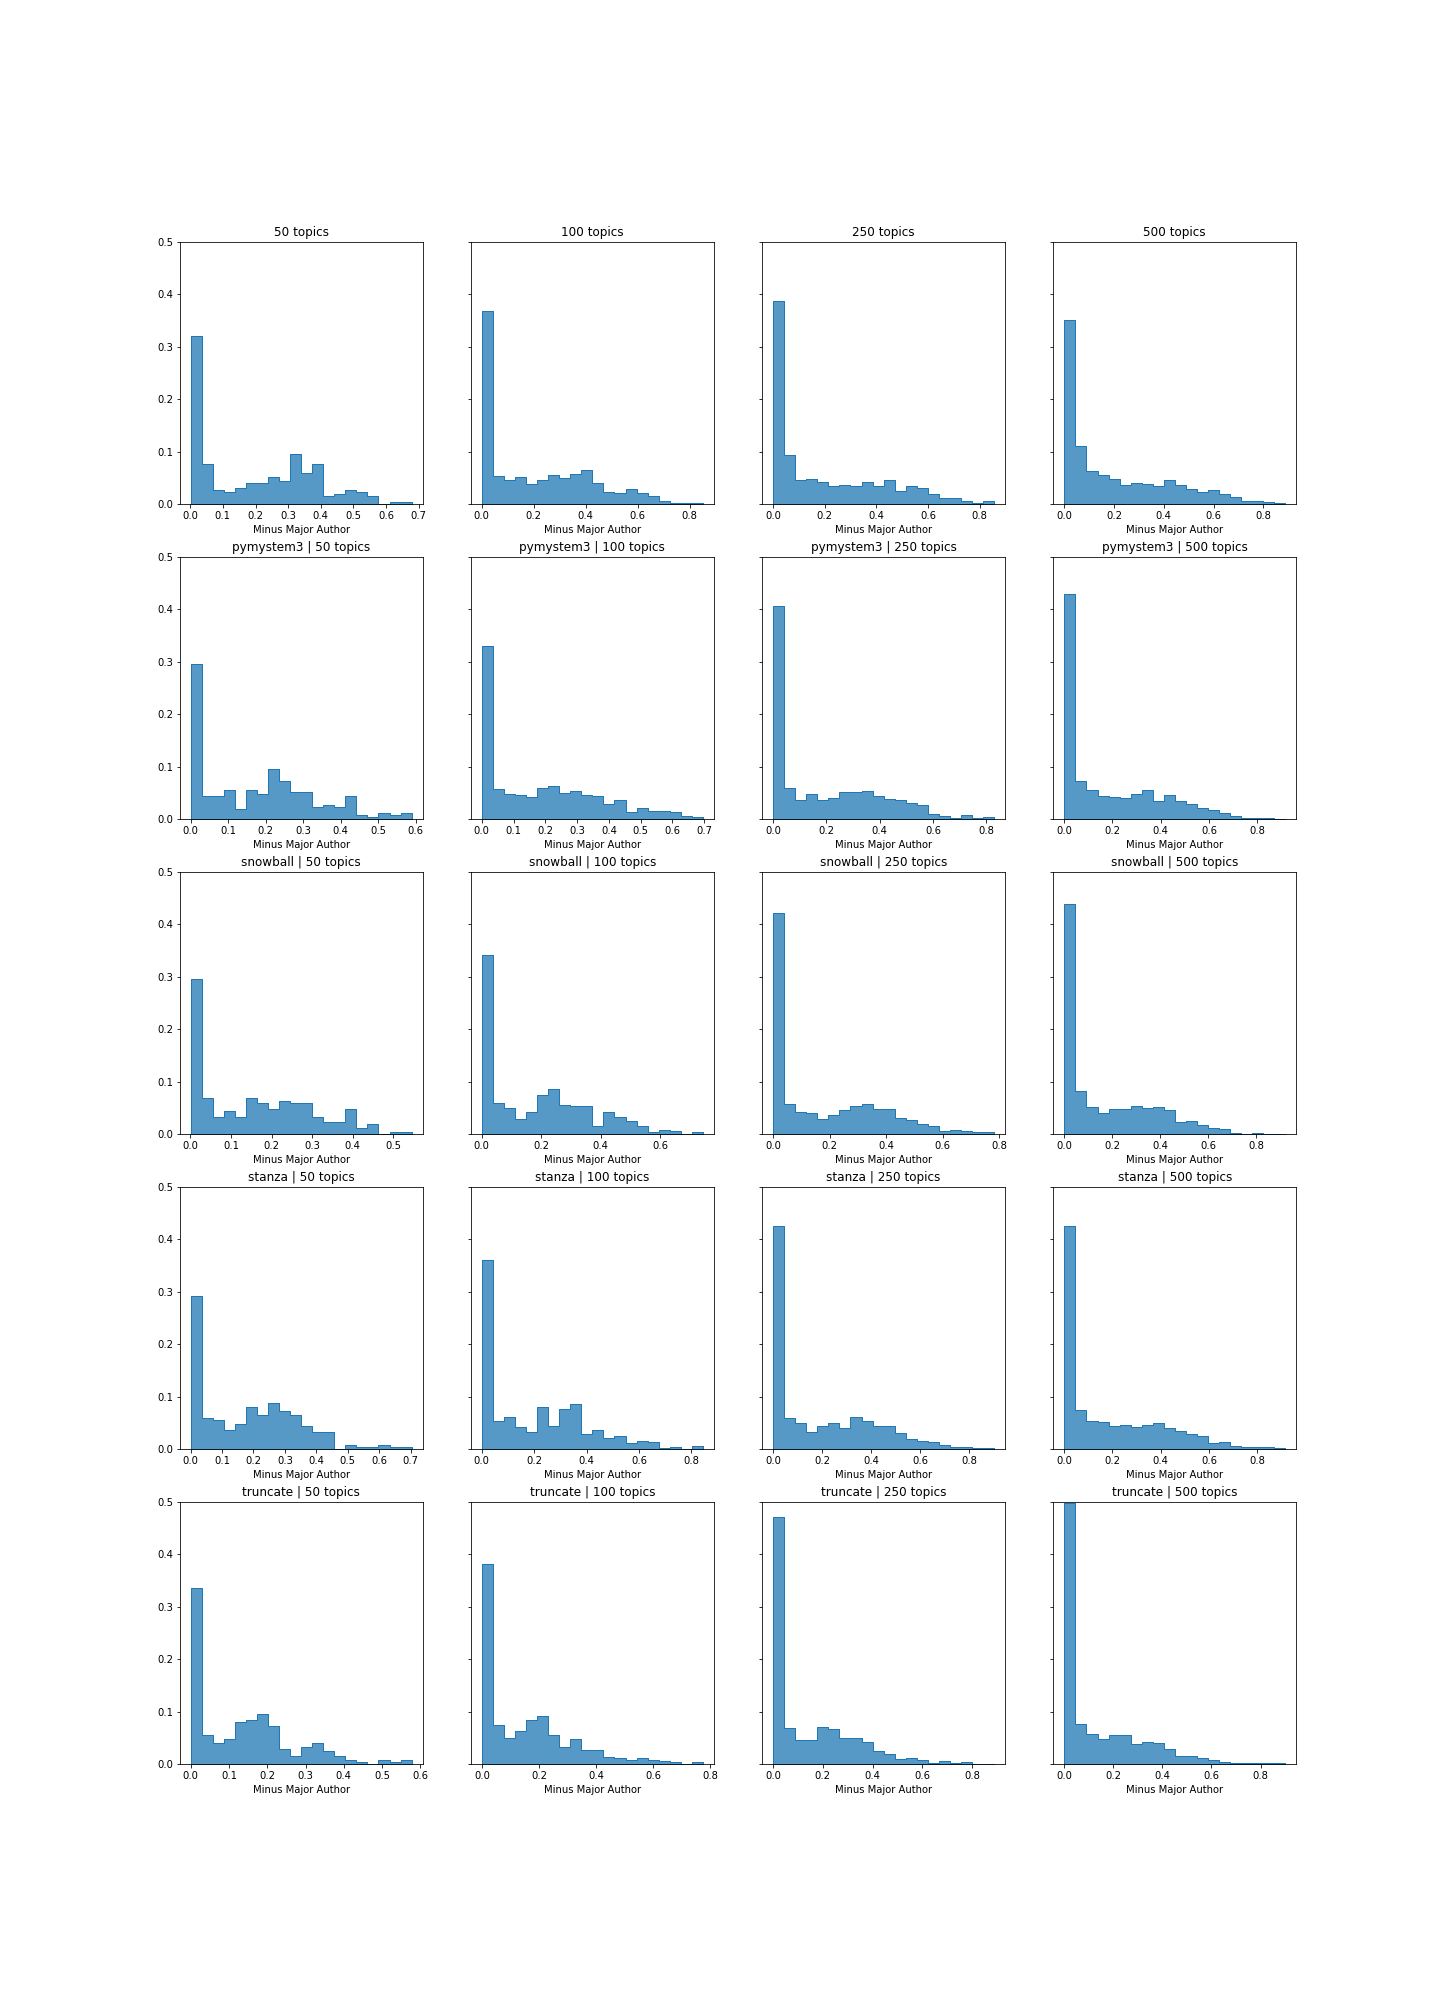
\includegraphics[width=\textwidth]{MinusMajorAuthor.png}
    \captionof{figure}{Author Entropy metric values for the 5 topic models trained for each number of topics $T \in \{50, 100,250, 500\}$, broken down by the number of topics and the type of conflation treatment used.}
    \label{fig:authorentropy}
\end{center}
\begin{center}
    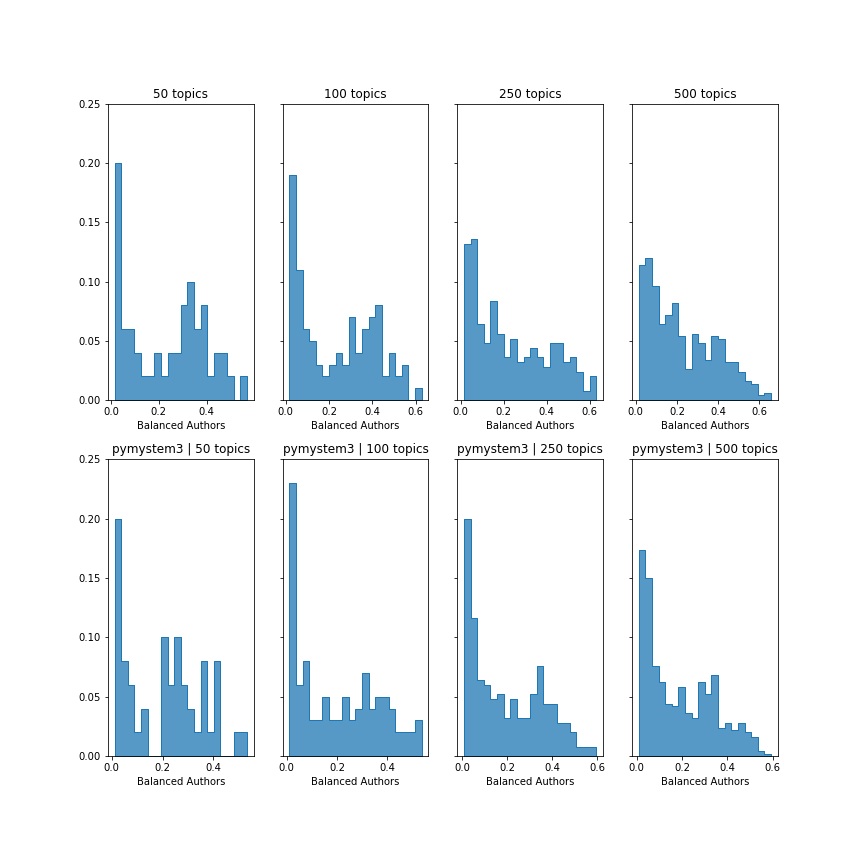
\includegraphics[width=\textwidth]{BalancedAuthors.png}
    %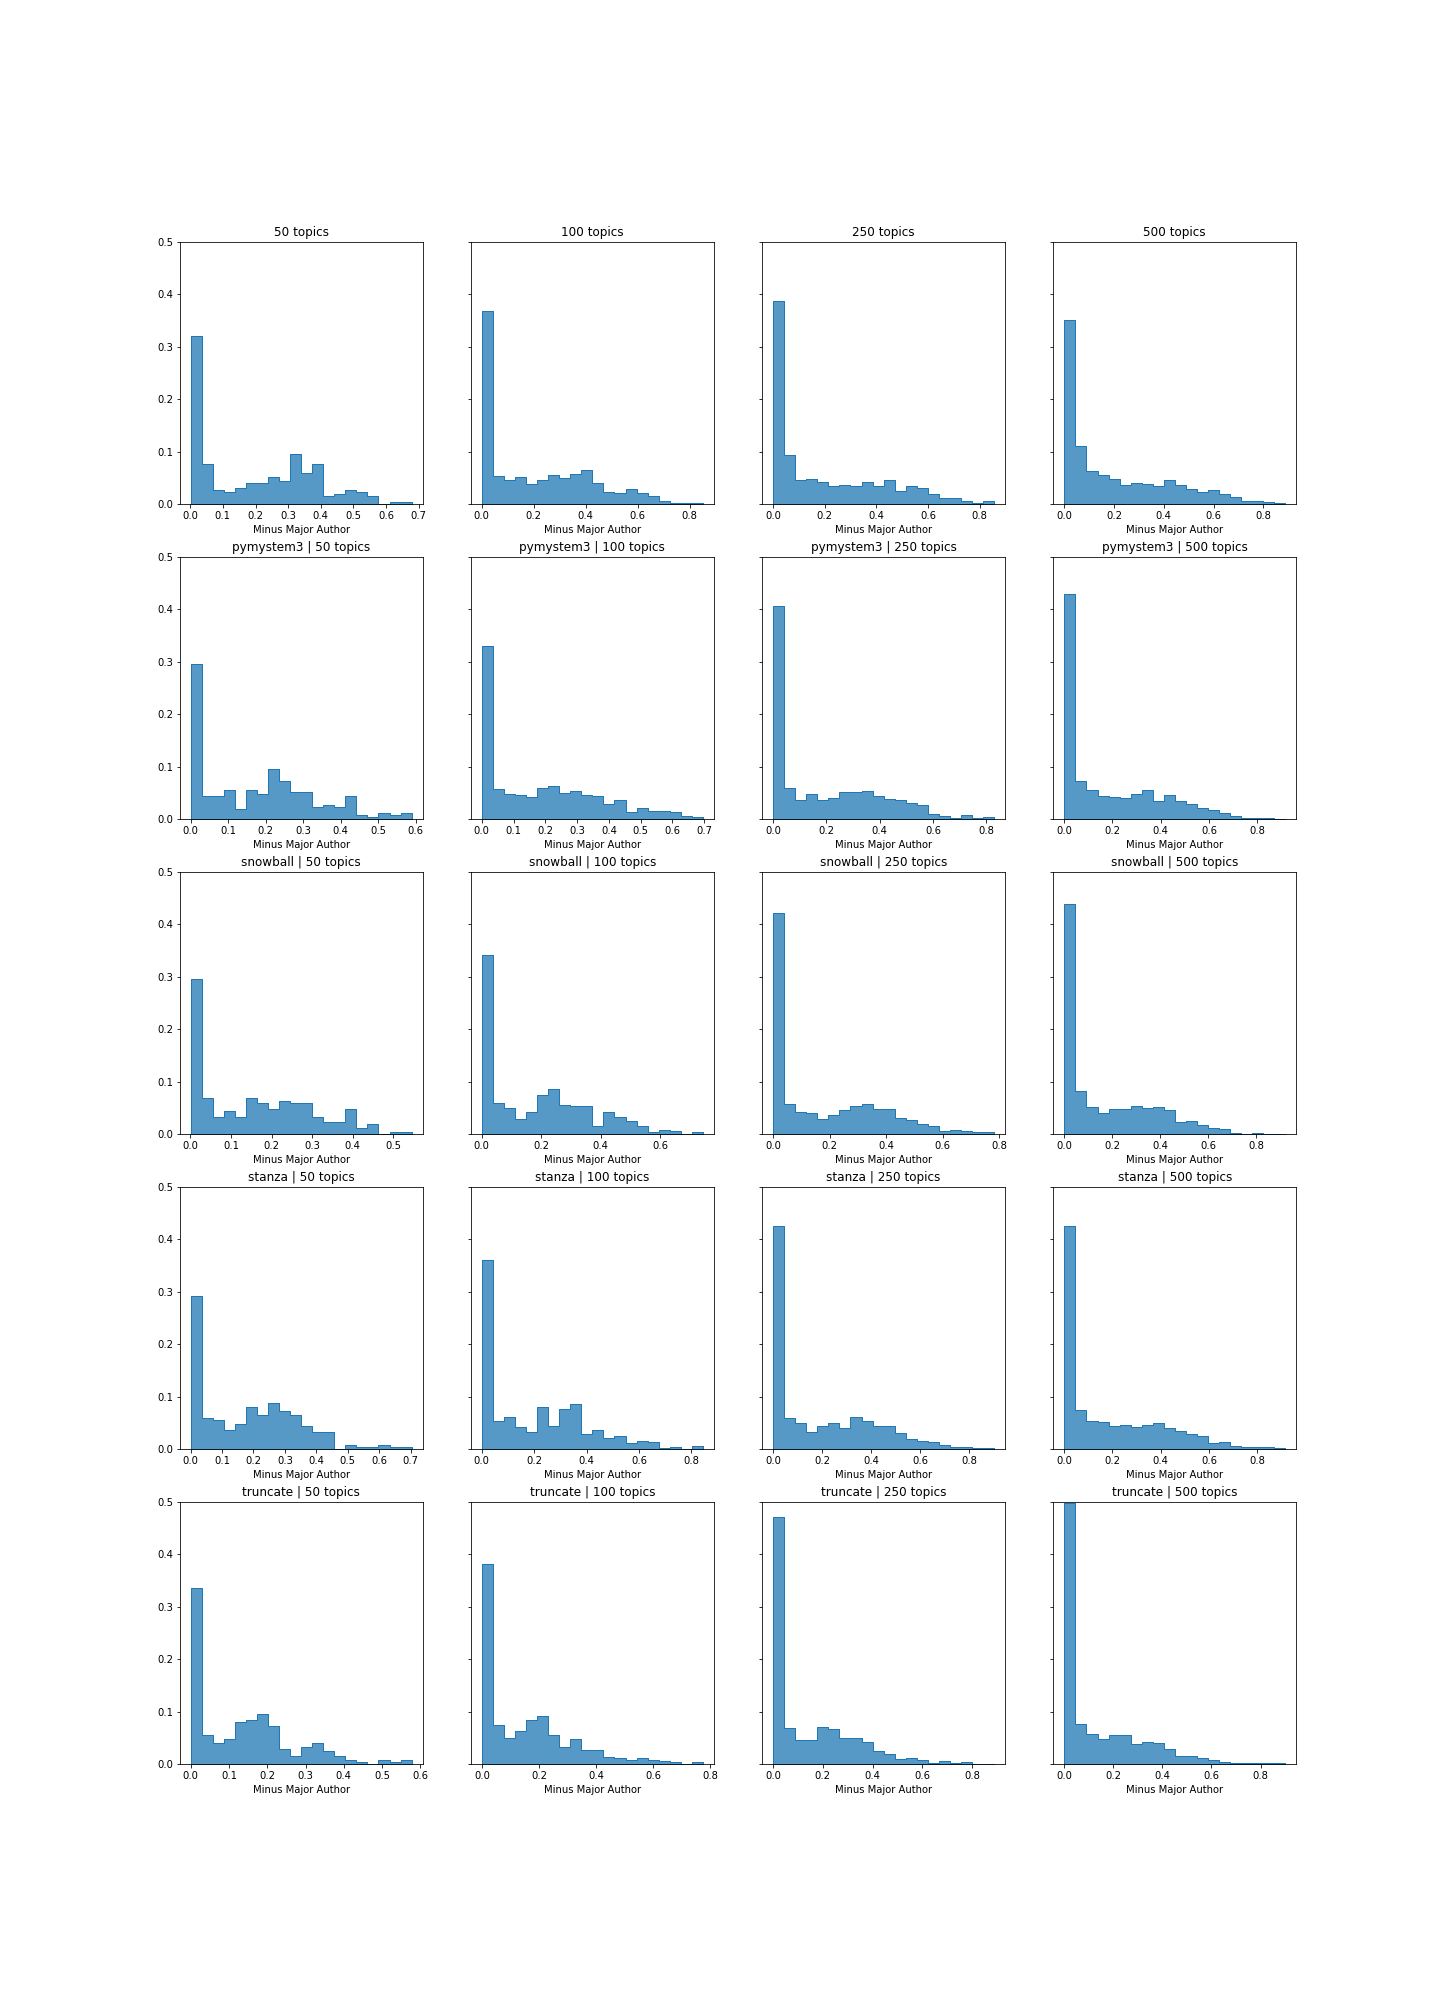
\includegraphics[width=\textwidth]{MinusMajorAuthor.png}
    \captionof{figure}{Balanced Author metric values for the 5 topic models trained for each number of topics $T \in \{50, 100,250, 500\}$, broken down by the number of topics and the type of conflation treatment used.}
    \label{fig:balauthor}
\end{center}
\begin{center}
    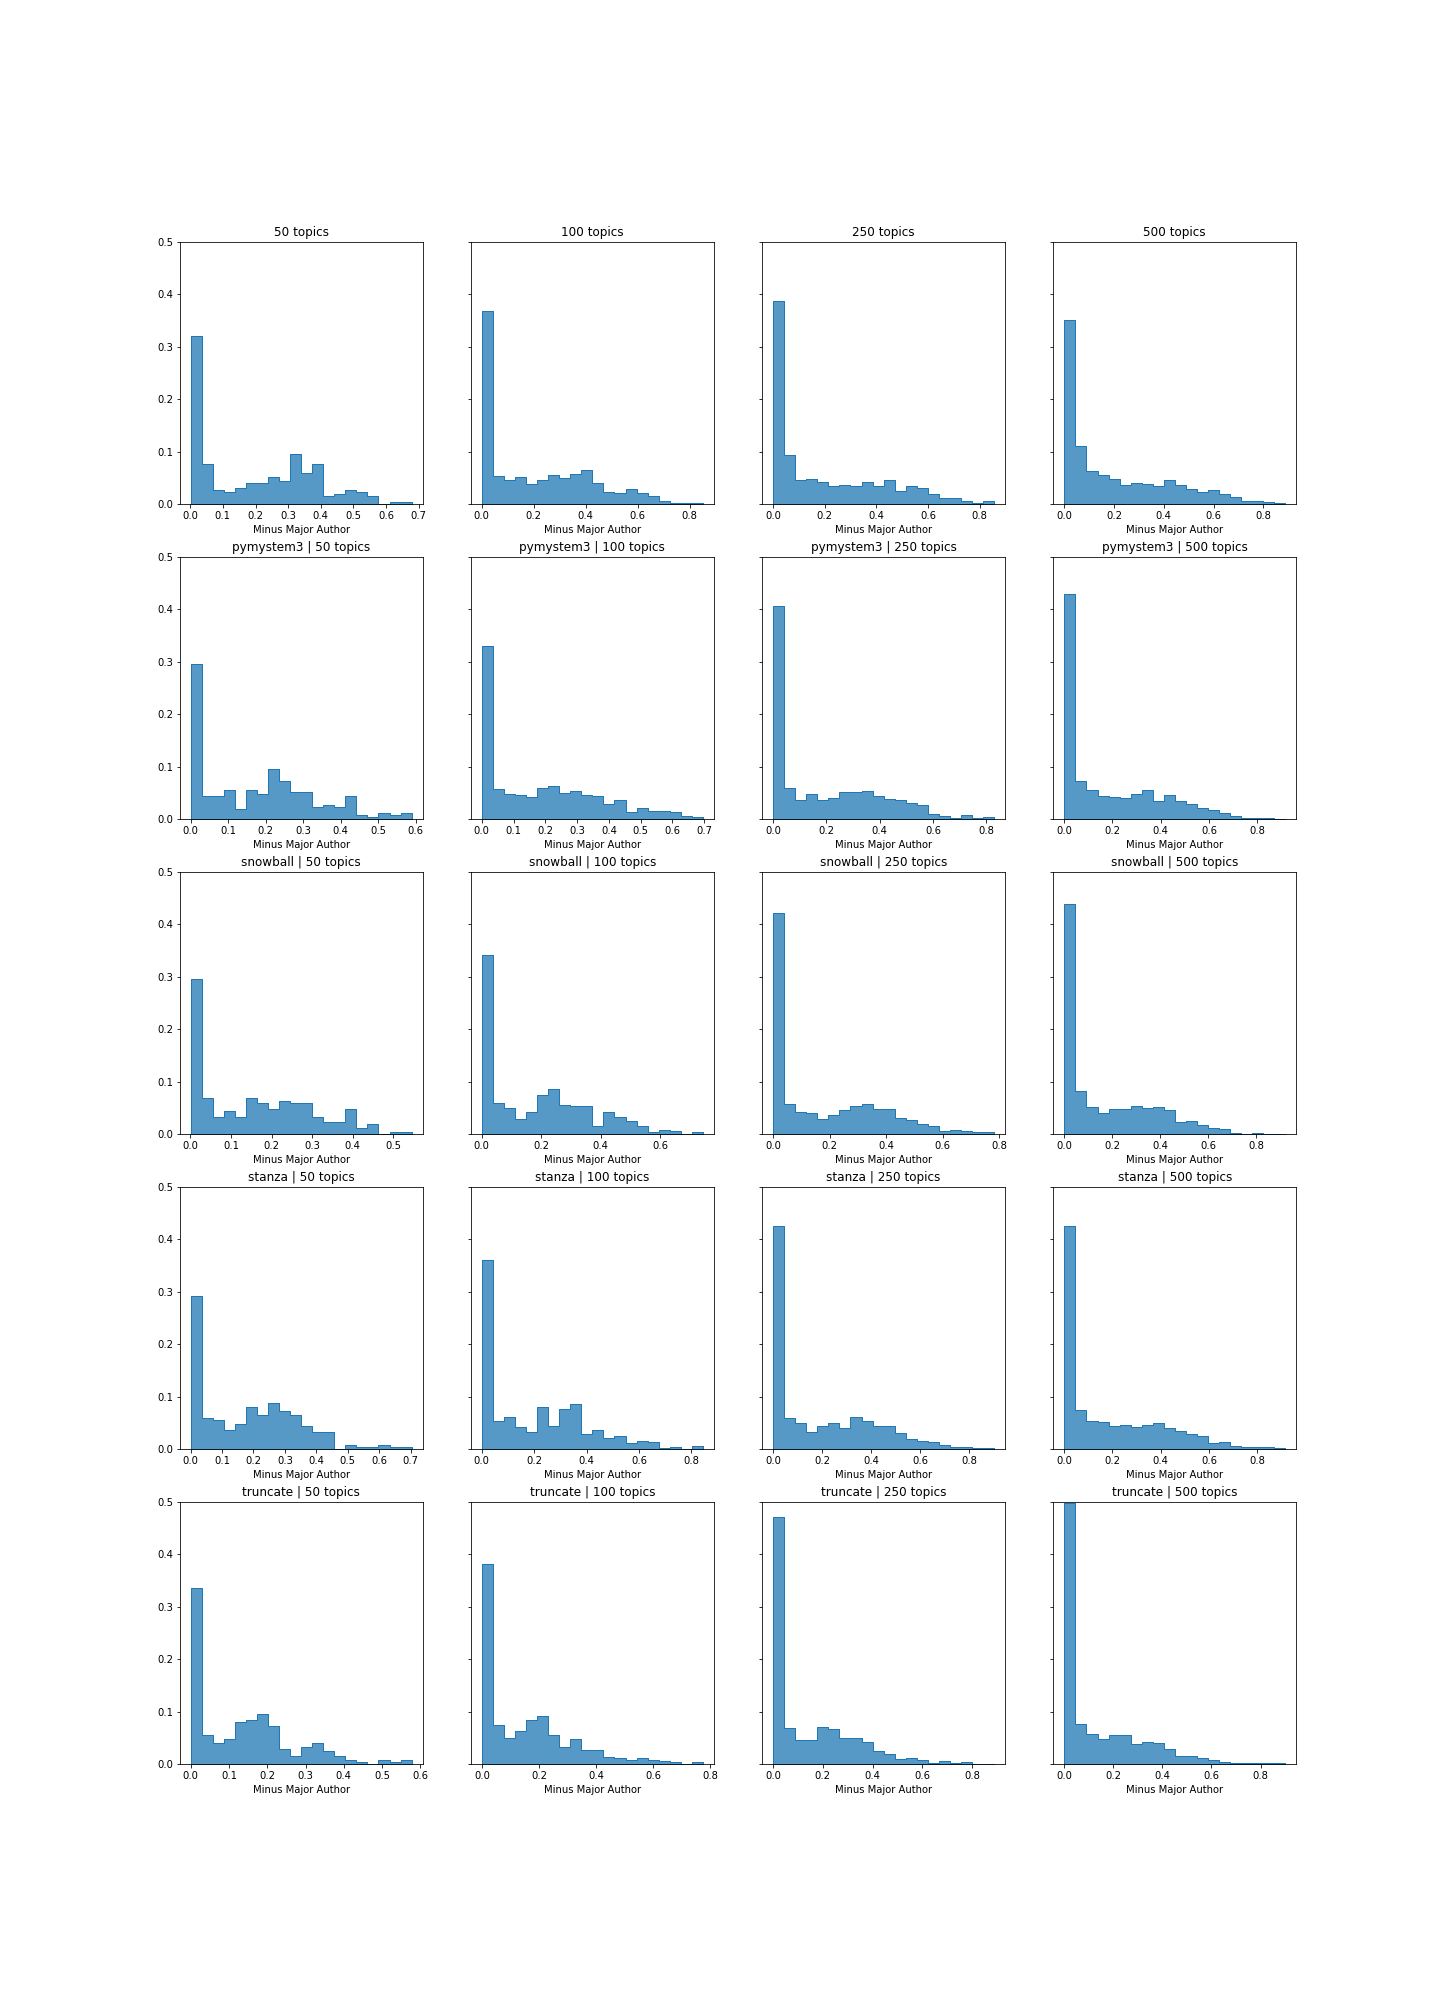
\includegraphics[width=\textwidth]{MinusMajorAuthor.png}
    \captionof{figure}{Minus Major Author metric values for the 5 topic models trained for each number of topics $T \in \{50, 100,250, 500\}$, broken down by the number of topics and the type of metrics  conflation treatment used.}
    \label{fig:mmauthor}
\end{center}
\pagebreak
\section{MALLET Diagnostics Metrics}
\begin{figure*}[!th]
    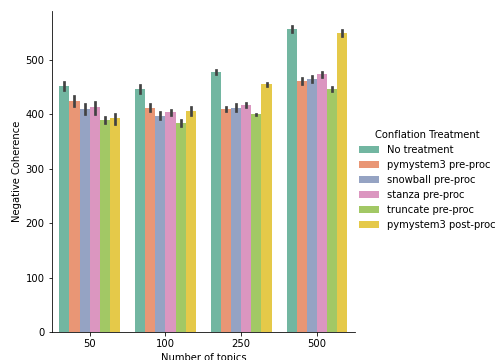
\includegraphics[width=0.5\textwidth]{negative_coherence.png}
    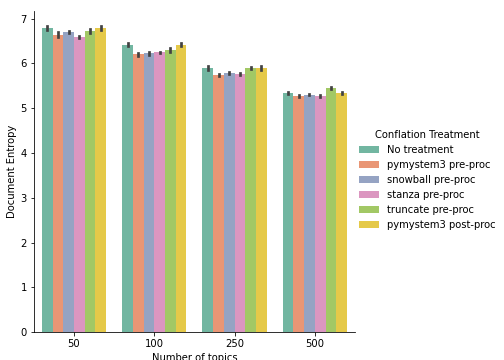
\includegraphics[width=0.5\textwidth]{document_entropy.png}
    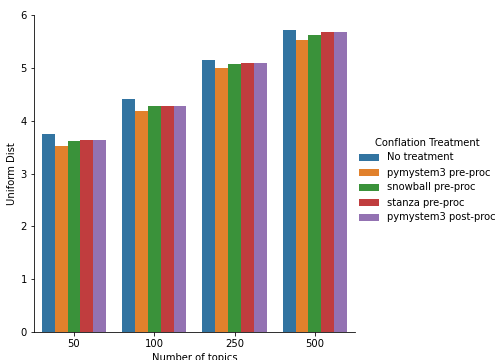
\includegraphics[width=0.5\textwidth]{uniform_dist.png}
    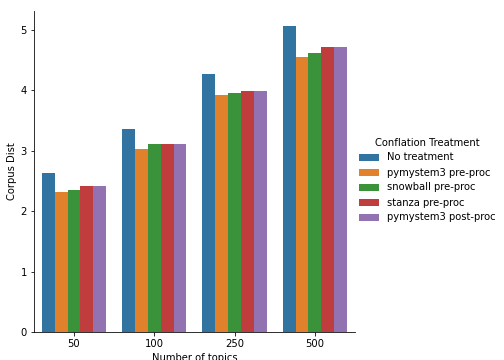
\includegraphics[width=0.5\textwidth]{corpus_dist.png}

    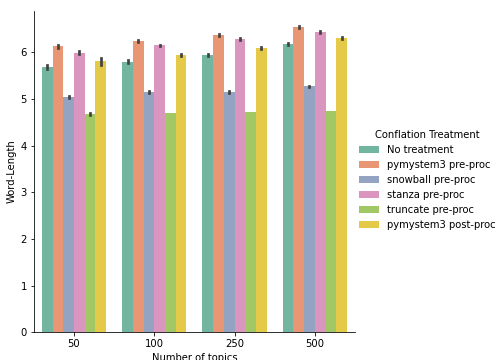
\includegraphics[width=0.5\textwidth]{word-length.png}
    \caption{Comparing averages over of metrics produced by MALLET between conflation treatments. These are mainly provided as a sanity check. Note that word-length is much higher for lemmatizers than stemmers, as expected.}
    \label{fig:mallet_metrics_figs}
\end{figure*}


\begin{landscape}
\thispagestyle{empty}
\newgeometry{left=2cm,top=1.5cm,textwidth=27.5cm,textheight=16.0cm, headheight=0.17573cm,headsep=0cm}
\onecolumn
\section{Morphological Analysis Produced by Lemmatizers}
\label{sec:appendix_morph}
\captionof{table}{Contrasting lemmatization and stemming outputs for various surface forms. Observe that Mystem output captures syncretism and that Stanza and Mystem return different lemmas for perfective verbs. Note that Mystem outputs are translated from Russian abbreviations.}
\label{table:verbaspect}

\begin{center}
%\begin{table*}[th]
    \centering
    \resizebox{\textwidth}{!}{\begin{tabular}{|l|l|l|l|l|}
    \hline
    \thead{\textbf{Surface}\\\textbf{form}} & \thead{\textbf{Translation and}\\\textbf{morphological features}} & \textbf{Mystem} & \textbf{Stanza} & \textbf{Snowball}\\\hline
    \foreignlanguage{russian}{ответ} & \thead{`answer' \\ Noun, Masculine, Singular, Inanimate \\Nominative or Accusative case} & \thead{\foreignlanguage{russian}{ответ}\\ Noun,Masc,Inan\\(Acc,Sing\textbar Nom,Sing)} & \thead{\foreignlanguage{russian}{ответ} \\Noun\\Animacy=Inan, Case=Nom, Gender=Masc, Number=Sing} & \foreignlanguage{russian}{ответ}\\\hline
    \foreignlanguage{russian}{ответим} & \thead{`we will answer/have answered' \\ Intransitive Verb, Perfective, 1st person, Plural, Future tense\\ Indicative or Imperative mood} & \thead{\foreignlanguage{russian}{отвечать}\\Verb,Intransive\\(Pl,Imperative,1st Pers,Perf\textbar NonPast,Pl,Indicative,1st Pers,Perf)} & \thead{\foreignlanguage{russian}{ответить} \\Verb\\Aspect=Perf, Mood=Ind, Number=Plur, Person=1, Tense=Fut, VerbForm=Fin, Voice=Act,} & \foreignlanguage{russian}{ответ} \\\hline
    \foreignlanguage{russian}{отвечать} & \thead{`to answer' \\ Intransitive Verb, Imperfective, Infinitive} & \thead{\foreignlanguage{russian}{отвечать}\\Verb,Intransive\\Inf,Imp} & \thead{\foreignlanguage{russian}{отвечать} \\Verb\\Aspect=Imp, VerbForm=Inf, Voice=Act,} & \foreignlanguage{russian}{отвеча}\\\hline
    \foreignlanguage{russian}{ответить} & \thead{`to answer'\\Intransitive Verb, Perfective, Infinitive} & \thead{\foreignlanguage{russian}{отвечать}\\Verb,Intransive\\Inf,Perf} & \thead{\foreignlanguage{russian}{ответить} \\Verb\\Aspect=Perf, VerbForm=Inf, Voice=Act,} & \foreignlanguage{russian}{ответ}\\\hline
    \foreignlanguage{russian}{большой} & \thead{`big' \\Adjective, Sing\\Masc, Animate: Nominative\\
    Masc, Inanimate: Nominative, Accuastive\\Fem: Genitive, Prepositional, Dative, Instrumental} & \thead{\foreignlanguage{russian}{большой}\\Adjective\\(Acc,Sing,Full,Masc,Inan\textbar Acc,Sing,Full,Masc,Inan\textbar Nom,Sing,Full,Masc\textbar \\Prep,Sing,Full,Fem\textbar Dat,Sg,Full,Fem\textbar Gen,Sing,Full,Fem\textbar Instr,Sing,Full,Fem)'} & \thead{\foreignlanguage{russian}{большой} \\Adjective\\Case=Nom,Degree=Pos,Gender=Masc,Number=Sing} & \foreignlanguage{russian}{больш}\\\hline
    \end{tabular}}

\end{center}
\pagebreak
\section{Comparison between untreated and post-stemmed topics}
\label{sec:sample_original_topics}
\captionof{table}{A selection of topics from a 100 topic model without any stemming treatment. Within a topic, surface forms with the same lemma are marked with the same color.}
\label{table:sample_original_topics}

\begin{center}
    \nopagebreak[4]
    \begin{tabularx}{\textwidth}{|l|X|l|l|l|l|l|X|}
    \hline
    \textbf{ID} & \textbf{Top 20 Keywords} & \thead{\textbf{Author}\\\textbf{Entropy}} & \thead{\textbf{Slot}\\\textbf{Entropy}} & \thead{\textbf{Lemma}\\\textbf{Entropy}} & \thead{\textbf{Slots to}\\\textbf{Keywords}} & \thead{\textbf{Lemmas to}\\\textbf{Keywords}} & \textbf{Comment} \\ \hline
    A & \foreignlanguage{russian}{\textcolor{orange}{клим} \textcolor{blue}{лидия} \textcolor{orange}{клима} \textcolor{magenta}{макаров} \textcolor{orange}{климу} варавка иноков спивак туробоев \textcolor{blue}{лидии} дронов лютов мать чтоб пред \textcolor{magenta}{макарова} дмитрий алина нею диомидов} & 0.1486 & 6.4539 & 8.6838 & 0.65 & 0.8 & Mostly names from \textit{The Life of Klim Samgin} by Maxim Gorky \\ \hline
    B & \foreignlanguage{russian}{\textcolor{orange}{цинциннат} м-сье пьер родион директор \textcolor{orange}{цинцинната} родриг \textcolor{orange}{цинциннату} иванович адвокат \textcolor{blue}{марфинька} \textcolor{magenta}{камере} роман стол эммочка дверь \textcolor{blue}{марфиньки} \textcolor{magenta}{камеры} библиотекарь \textcolor{magenta}{камеру}} &  0.1926 & 6.1703 & 8.2002 & 0.7 & 0.8 & Names and themes from \textit{Inviation to a Beheading} by Vladimir Nabokov\\ \hline
    C & \foreignlanguage{russian}{\textcolor{magenta}{солнце} небо \textcolor{orange}{сад} ветер \textcolor{blue}{воды} \textcolor{magenta}{солнца} берегу казалось вокруг здесь \textcolor{teal}{землю земли} \textcolor{blue}{вода} ними воздух далеко тени лес около \textcolor{orange}{саду}} & 2.5730 & 6.3960 & 9.7248 & 0.7 & 0.8 &  Words about nature: `sun', `river', `garden', `water', `riverbank', `sky', `forest',`earth'\\ \hline
    D & \foreignlanguage{russian}{говорила сама спросила стала думала хотела могла нею знала начала мать продолжала одна пошла вышла видела сидела встала села смотрела} & 2.7266 & 6.0929 & 9.6380 &  0.5 & 1 & The feminine reflexive pronoun `herself', `mother', and many past tense feminine verbs: `talked', `asked', `became', `wanted', `thought'...\\ \hline
    E & \foreignlanguage{russian}{фр de la vous le et un je a франц c'est mon pas que il les англ mais est ma} & 1.8941 & 3.8524 & 4.9799 & 0.15 & 0.15 & French words and `France'. \\ \hline
    F & \foreignlanguage{russian}{\textcolor{orange}{говорит говорю} смотрит стоит идет видит кричит спрашивает сидит отвечает глядит девица начинает лежит берет молчит хочет бежит плачет слышит} & 2.5775 & 5.8909 & 9.3936 & 0.4 & 0.95 & Mainly verbs about talking and interacting, nearly all in the 3rd person. \\ \hline
    G & \foreignlanguage{russian}{\textcolor{blue}{петрович} \textcolor{orange}{базаров} аркадий николай павел василий иванович анна сергеевна \textcolor{blue}{петровича} промолвил евгений одинцова катя \textcolor{orange}{базарова} фенечка аркадия заметил аркадию франц} & 0.7604 & 6.2496 & 8.2076 & 0.55 & 0.85 & Nearly all names and patronymics with two past tense masculine verbs, `uttered' and `noticed'. \\ \hline
    H & \foreignlanguage{russian}{продолжал \textcolor{blue}{ответил} начал проговорил посмотрел нему \textcolor{orange}{голосом голос} встал подошел глазами заметил заговорил улыбнулся \textcolor{blue}{отвечал} сел прибавил обратился тотчас сейчас} & 2.5037 & 6.2502 & 9.4994 & 0.5 & 0.9 & `Voice' and past tense masculine verbs of talking and interacting: `continued', `began', `spoke', `looked'... \\ \hline
    \end{tabularx}

\end{center}
\begin{center}
\begin{tabularx}{\textwidth}{|l|X|l|l|l|l|l|X|}\hline
    I & \foreignlanguage{russian}{\textcolor{orange}{моей моя мое моего мои мою} ко \textcolor{orange}{мною моих} сердце \textcolor{orange}{моим мной моем} \textcolor{blue}{жизни} нам \textcolor{orange}{моему} сердца могу \textcolor{blue}{жизнь} наши} & 2.5911 & 6.8899 & 8.6942 & 0.9 & 0.4 & The first person possessive pronoun \foreignlanguage{russian}{\textcolor{orange}{мой}} `my' repeated many times. The words `life' and `heart' also appear.  \\ \hline
    J & \foreignlanguage{russian}{\textcolor{orange}{мальчик} \textcolor{blue}{учитель} \textcolor{orange}{мальчика} \textcolor{magenta}{учителя} \textcolor{olive}{детей} \textcolor{teal}{школы} \textcolor{olive}{дети} лет \textcolor{orange}{мальчики мальчишка} \textcolor{teal}{школе} \textcolor{orange}{мальчиков} классе гимназии \textcolor{teal}{школу} \textcolor{red}{уроки} девочка \textcolor{red}{урок} \textcolor{olive}{ребенок} товарищей} & 2.3820 & 6.7395 & 8.8690 & 0.7 & 0.55 & A topic about school, but \foreignlanguage{russian}{\textcolor{orange}{мальчик}} `boy' is repeated. The other repeated words are `teacher', `lesson, `child'. \\ \hline
\end{tabularx}
\end{center}


\begin{center}
\captionof{table}{The same topics from table \ref{table:sample_original_topics} but with post-stemming applied}
\label{table:post_stem_topics}

\begin{tabularx}{\textwidth}{|l|X|l|l|l|l|l|X|}
    \hline
    \textbf{ID} & \textbf{Top 20 Keywords} & \thead{\textbf{Author}\\\textbf{Entropy}} & \thead{\textbf{Slot}\\\textbf{Entropy}} & \thead{\textbf{Lemma}\\\textbf{Entropy}} & \thead{\textbf{Slots to}\\\textbf{Keywords}} & \thead{\textbf{Lemmas to}\\\textbf{Keywords}} & \textbf{Comment} \\ \hline
    % post stemming
    A-post & \foreignlanguage{russian}{клим лидия макаров варавка инок спивак дронов мать туробой алина дмитрий диомидов томилин лют чтоб маракуев пред дядя нехаева девушка} & 0.1486 & 4.5456 & 8.6617 & 0.5 & 1 & Mostly names from \textit{The Life of Klim Samgin} by Maxim Gorky \\\hline
    B-post & \foreignlanguage{russian}{цинциннат пьер м-сье родион директор родрига камера марфинька иванович адвокат стол койка эммочка роман стул крепость дверь библиотекарь давать казнь} & 0.1926 & 4.1709 & 8.1850 & 0.45 & 1 & Names and themes from \textit{Invitation to a Beheading} by Vladimir Nabokov\\ \hline
    D-post & \foreignlanguage{russian}{спрашивать говорить становиться сам мать один она думать отвечать муж выходить мочь хотеть пойти улыбаться начинать знать голос продолжать свой} & 2.7266 &  4.4762 & 9.6360 & 0.6 & 1 & The stemmed version of D, but all verbs are now infinitive forms, so the feminine subject information is lost. \\ \hline
    E-post & \foreignlanguage{russian}{фр de la vous le et un je a франц c'est mon pas que il les англ mais est ma } & 1.8941 & 2.8536 & 4.9795 & 0.15 & 0.15 & French words and `France'.\\\hline
    F-post & \foreignlanguage{russian}{говорить стоять кричать идти смотреть сидеть спрашивать глядеть видеть отвечать слышать девица начинать лежать плакать бежать смеяться ходить приходить берет} & 2.5775 & 4.5224 & 8.5917 & 0.55 & 1 & Mainly verbs about talking and interacting, nearly all in the 3rd person. \\ \hline
    G-post & \foreignlanguage{russian}{петрович базаров аркадий николай павел василий анна сергеевна иванович промолвить катя евгений одинцова фенечка петр замечать брат отец франц отвечать } & 0.7604 & 4.5113 & 8.1489 & 0.5 & 1 & Nearly all names and patronymics, plus three verbs `to utter', `to notice', `to answer,' and two common nouns, `father' and `brother'.\\ \hline
\end{tabularx}
    \end{center}
\begin{center}
\begin{tabularx}{\textwidth}{|l|X|l|l|l|l|l|X|}\hline

    H-post & \foreignlanguage{russian}{свой отвечать голос лицо улыбаться продолжать глаз стол садиться начинать вставать обращаться говорить подходить посмотреть улыбка хотеть проговаривать замечать взгляд } & 2.5037 & 4.3617 & 9.5059 & 0.45 & 1 & Possessive pronoun \foreignlanguage{russian}{свой}, some common nouns, `voice', `face', `eye', `table', `smile', and many verbs about interacting, `to answer', `to continue', `to begin', etc...\\ \hline
    I-post & \foreignlanguage{russian}{мой наш сердце я жизнь ко мы мочь любовь твой слеза душа один год имя свет быть видеть леон друг} & 2.5911 & 4.3650 & 8.6968 &  0.7 & 1 & These are very common words, particularly pronouns, but also `love', `tears', `soul', `name' and the infinitive forms of `to be' and `to see'.\\ \hline
    J-post & \foreignlanguage{russian}{мальчик учитель ребенок школа урок мальчишка класс девочка товарищ учиться год гимназия ученик маленький учить мальчиков директор училище взрослый отец} & 2.3820 & 3.9490 & 8.8672 & 0.45 & 0.95 & More words related to school children are visible after post-stemming, `to study', `year', `student', `little', `principal', `adult', `father'. \\ \hline
    \end{tabularx}
\end{center}
\pagebreak

\section{Topics from models trained on preprocessed data}
\label{sec:preprocessed_topics}
\captionof{table}{These are sample topics from models with 100 topics trained on various preprocessed versions of the corpus. We see interpretable topics that are both author specific and general. Words within the same topic that likely share a lemma are highlighted in the same color. The aggressive, simpler stemmers do not conflate these because they cannot capture consonant alternation patterns in Russian verb conjugations. }
\begin{center}
    \begin{tabularx}{\textwidth}{|l|X|l|l|X|}
    \hline
    \textbf{ID} & \textbf{Top 20 Keywords} & \textbf{Treatment} & \textbf{Author Entropy} &  \textbf{Comment} \\ \hline
    K & \foreignlanguage{russian}{логин анна клавдия мотовилов андозерский шестов валя молин мальчик город ж баглаев ермолин коноплев юшка шест дубицкий крикунов гомзин заговаривать} & Mystem & 0.149863 & Mostly names from \textit{Bad Dreams} by Fyodor Sologub, but also 'boy', 'city' \\ \hline
    L & \foreignlanguage{russian}{цинциннат м пьер сье родион директор родрига марфинька камера иванович адвокат эммочка койка стена роман друг стул паук крепость проговаривать} & Mystem & 0.1779 & Names and themes from \textit{Invitation to a Beheading} by Vladimir Nabokov \\ \hline
    M & \foreignlanguage{russian}{слеза сердце плакать бросаться подходить тихо ужас сила умирать упасть грудь бледный вставать прощать останавливаться слышать быстро дрожать подымать бросать} & Mystem & 2.7315 & Words about sadness: `tears', `heart', `to cry', `to throw oneself', `horror', `strength' \\ \hline
    N & \foreignlanguage{russian}{сад дерево лес цветок солнце трава лист белый зеленый куст старый тень дорожка поле здесь земля аллея гора зелень скамейка} & Mystem & 2.6638 & Words about nature: `garden', `tree', `flower', `sun', `grass', `leaf,' `white', `green' \\ \hline
    O & \foreignlanguage{russian}{прокуратор пилат иуда иешуа город левий гость ершалаим сад арестант секретарь афраний игемон балкон столб дворец матвей луна дорога солнце} & Stanza & 0.34331 & Words related to biblical themes: `Pontius Pilate', `Judea`, `Jerusalem', `garden'. This is a topic highly correlated with Mikhail Bulgakov from imagery in \textit{Master and Margarita}. \\ \hline
    P & \foreignlanguage{russian}{вода солнце лес берег дерево дорога сад белый небо река земля трава далеко куст поле гора зеленый лист ветер старый} & Stanza & 2.5371 & Words about nature: `water', `sun', `riverbank', `tree' \\ \hline
    Q & \foreignlanguage{russian}{генерал город чиновник имя петербург губерния губернатор губернский помещик служба служить сын дворянин весьма господин чин русский советник мундир предводитель} & Stanza & 2.5535 & Words about the civil service and governance: `general', `city', `official', `Petersburg', `province', `governor', `service' \\ \hline
    R & \foreignlanguage{russian}{письм \textcolor{orange}{писа написа} бумаг записк чита получ \textcolor{orange}{пишет} конверт пер переда взял \textcolor{orange}{пиш} лист бумажк строк буд соб \textcolor{blue}{прочел почерк}} & Snowball & 2.5884 & Stems about writing, sending and reading letters. \\ \hline
    \end{tabularx}
\end{center}
    \begin{tabularx}{\textwidth}{|l|X|l|l|X|}\hline
    S & \foreignlanguage{russian}{клим лид самгин варавк макар лют алин инок спивак туробо дрон варвар дмитр макаров томилин пред дьякон девушк брат снов} & Snowball & 0.1525 & Names from \textit{The Life of Klim Samgin} by Maxim Gorky \\ \hline
    T & \foreignlanguage{russian}{самги варва марин клим снова револ дроно тагил пред чтоб безбе толст кутуз ивано затем любаш дуняш чорт пробо вспом} & Truncate & 0.1981 & Names from \textit{The Life of Klim Samgin} by Maxim Gorky with some roots of common words mixed in. \\ \hline
    U & \foreignlanguage{russian}{лошад мужик кучер коляс крыль подъе телег прика стари экипа поеха колес барин ехать извоз запря приех станц бричк карет} & Truncate & 2.5469 & Roots about traveling, `horse', `coachman', `wheel'. \\ \hline
    V & \foreignlanguage{russian}{письм бумаг запис \textcolor{orange}{напис писал} получ \textcolor{orange}{писат} бумаж кабин карма подпи проче доста проси конве посла \textcolor{orange}{пишет} стол читат адрес} & Truncate & 2.6027 & Roots about writing and letters. \\ \hline
    \end{tabularx}
%\end{center}

\end{landscape}

\end{document}
